\chapter[Analysis]{Analysis}

\section{Overview}
While Figure \ref{fig:alldata-GOES6-1983-1991} shows an overview of the most pertinent variables used in this study, some further analysis was done to determine any potential biases introduced by specifics of the satellite motion or derivations used. For example, Figure \ref{fig:ByHourExample} shows that not only did data availability vary significantly with local time, but the values themselves vary significantly. \vinote{Cite that this is known (dawn vs dusk, etc)}

\begin{figure}
\centering
\includegraphics[width=0.7\linewidth]{Figures/rhoLT.eps}
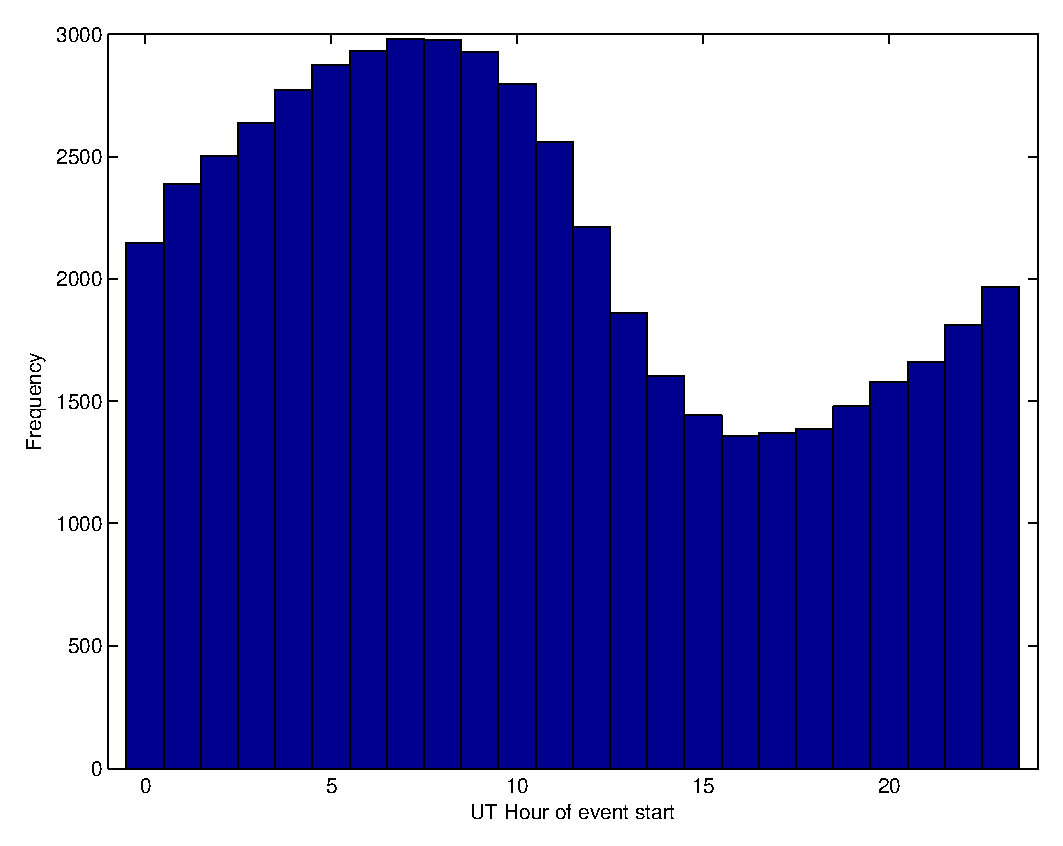
\includegraphics[width=0.7\linewidth]{Figures/nansbyhour.eps}
\caption{Median \req\ binned by local time, and availability of \req\ with local time.}
\label{fig:ByHourExample}
\end{figure}

This trend similarly holds for Magnetic Local Time (MLT), a time basis where "noon" points directly magnetically upstream in the solar wind. \vinote{Does it even make sense to compare \req\ to local time?}  

\section{$F_{10.7}$ Dependence}
\cite{Takahashi2010SolarCycleVariation} showed a strong correlation between the 27-day averaged $F_{10.7}$ index of solar activity and the averaged equatorial mass density (\req). This was chosen as a starting place for verifying the data analysis routines developed for this dataset, so as to show that data input, averaging, and interpolation were all done in a reasonable and reproducible manner. Figure \ref{fig:F107rhoeq27dcomparison} shows the strong correlation seen previously, and reasonably reproduces Figure 13.b from \cite{Takahashi2010SolarCycleVariation} for the years covered by GOES 6.

\begin{figure}
\centering
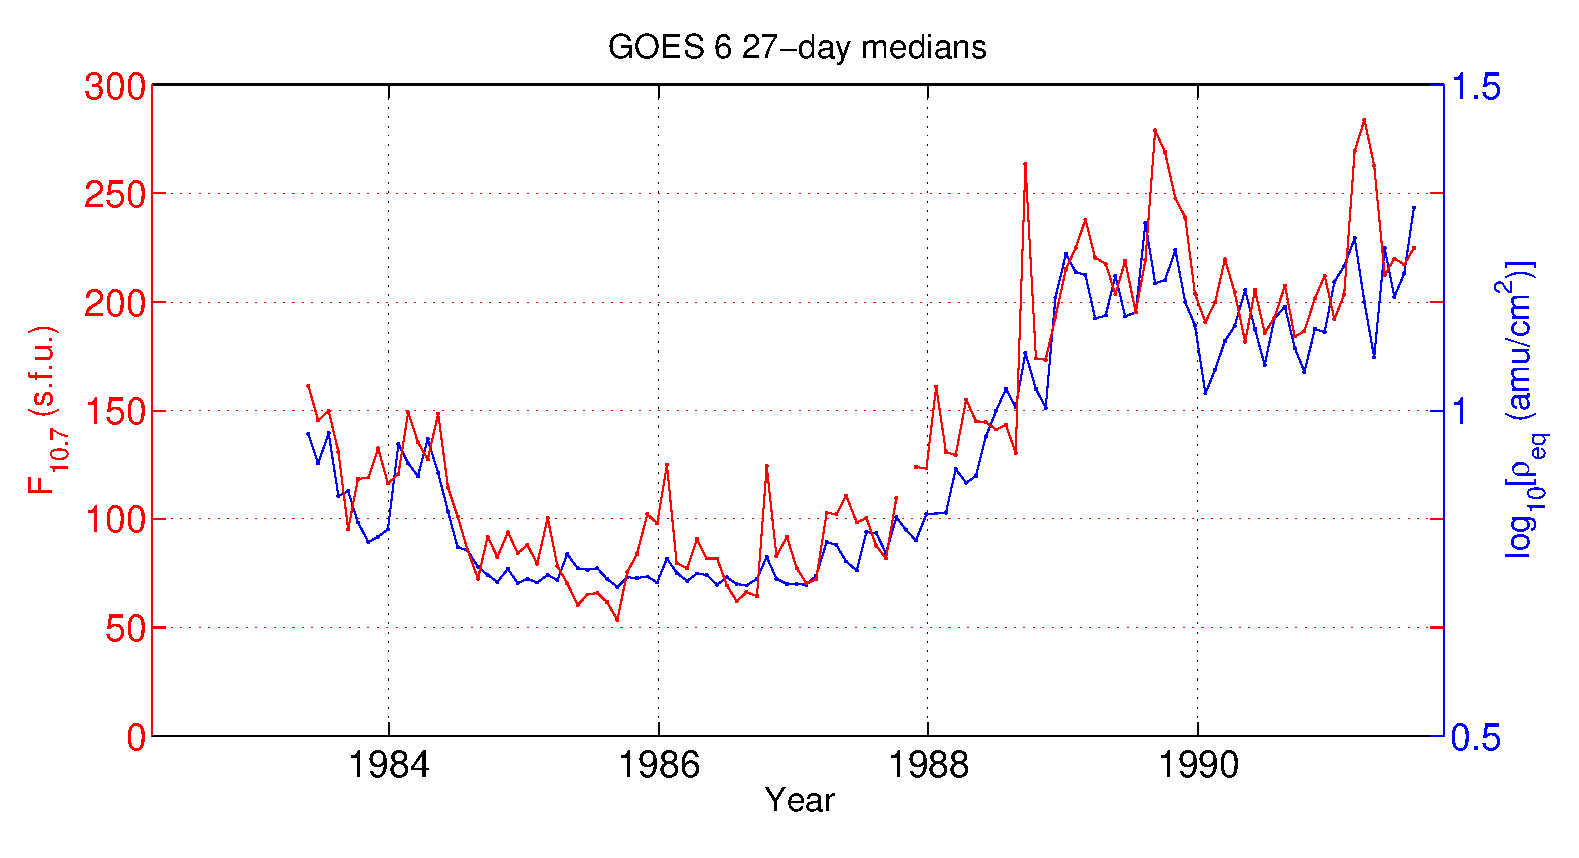
\includegraphics[width=0.7\linewidth]{Figures/F107MD27d-GOES6}
\caption{Comparing $F_{10.7\_27d}$ and $log(\rho_{eq\_27d})$ using GOES 6 data}
\label{fig:F107rhoeq27dcomparison}
\end{figure}

\section{Linear Correlations}
This dependence was further investigated, and extended, by creating a simple one-time-lag linear model for each major variable in the database as well as combinations of some to test for independent contributions to the correlation. The models were trained on half of the dataset and tested on the other half for each satellite, and this was repeated with new random samples 100 times and then the median correlation values were taken. The results are shown in Table \ref{CCperltable}.

\begin{table}[h]
	\small
	\begin{tabular}{|l|llll|}
		\hline
		& GOES 2 & GOES 5 & GOES 6 & GOES 7\\ \hline
		doy & -0.08 & +0.10 & -0.05 & +0.06 \\
		MLT & -0.09 & -0.09 & -0.04 & -0.05 \\
		Bz & +0.17 & -0.12 & +0.08 & -0.08 \\
		Vsw & -0.04 & +0.29 & +0.06 & -0.06 \\
		Dst & +0.27 & +0.66 & +0.06 & +0.22 \\
		Rhosw & +0.34 & +0.63 & +0.07 & +0.34 \\
		F107 & +0.42 & +0.14 & +0.49 & +0.42 \\
		Bz+Vsw & +0.09 & +0.19 & +0.12 & -0.11 \\
		Dst+F107 & +0.45 & +0.69 & +0.53 & +0.47 \\
		All & -0.10 & +0.34 & +0.61 & +0.39 \\
		\hline
	\end{tabular}
	\caption{Table of linear model correlations showing the median of 100 random samples. Each sample trained on half of the data (via randomly selected rows of the least squares matrix) and tested on the other half} 
	\label{CCperltable}
\end{table}

\vnote Look at making this (along with figures) a git submodule

It can be seen that $F_{10.7}$ almost always correlates the most with \req, but that there is significant variance between data from different satellites. \vinote{Including training correlations? Make model a 12 hour model to smooth it out a bit?}

\section{Nonlinear Correlations}

Similarly for a simple neural net model with one time lag, Table \ref{NNperltable}

\begin{table}[h]
	\small
	\begin{tabular}{|l|llll|}
		\hline
		& GOES 2 & GOES 5 & GOES 6 & GOES 7\\ \hline
		doy & +0.20 & +0.31 & +0.13 & +0.11 \\
		MLT & +0.18 & +0.12 & +0.16 & +0.10 \\
		Bz & +0.14 & +0.23 & +0.07 & +0.05 \\
		Vsw & +0.14 & +0.24 & +0.07 & +0.06 \\
		Dst & +0.16 & +0.05 & +0.11 & +0.10 \\
		Rhosw & +0.17 & +0.17 & +0.32 & +0.14 \\
		F107 & +0.33 & +0.29 & +0.50 & +0.38 \\
		Bz+Vsw & +0.17 & +0.26 & +0.10 & -0.04 \\
		Dst+F107 & +0.22 & +0.20 & +0.45 & +0.34 \\
		All &  &  &  &  \\
		\hline
	\end{tabular}
	\caption{Table of nonlinear model correlations showing the median of 100 random samples. Each sample trained on half of the data (via randomly selected rows of the least squares matrix) and tested on the other half} 
	\label{NNperltable}
\end{table}
